\documentclass [11pt]{articleSBPO}

\usepackage[brazil]{babel}
\usepackage[utf8]{inputenc}
\usepackage[T1]{fontenc}
\usepackage{graphics}
\usepackage[a4paper,top=3.3cm,left=2.9cm,right=2.9cm,bottom=2.5cm,noheadfoot]{geometry}
\usepackage{algorithm}
\usepackage{algorithmic}
\usepackage{times}
\usepackage{amsmath}
\usepackage{amssymb}
\usepackage{setspace}
\usepackage{graphicx}
\usepackage{subfig}
\usepackage{indentfirst}
\usepackage{icomma}
\usepackage{url}
\usepackage{longtable}
\usepackage{lscape}
\usepackage{array}
\usepackage[alf]{abntex2cite}
\usepackage{epstopdf}
\usepackage{rotating}
\newcommand{\up}[1]{\raisebox{1.3ex}[0pt]{#1}}
% \usepackage{latex8}
\floatname{algorithm}{Algoritmo}
\def\figurename{Figura}
\def\tablename{Tabela}

%%%%%%%%%%%%%%%%%%%%%%%%%%%%%%%%%%%%%%%%%%%%%%
%     configurações do pacote algorithm
%%%%%%%%%%%%%%%%%%%%%%%%%%%%%%%%%%%%%%%%%%%%%
% \renewcommand{\algorithmcfname}{alg}
\floatname{algorithm}{Algoritmo}
\renewcommand{\algorithmicrequire}{\textbf{Entrada:}}
\renewcommand{\algorithmicensure}{\textbf{Saída:}}
\renewcommand{\algorithmicend}{\textbf{fim}}
\renewcommand{\algorithmicif}{\textbf{se}}
\renewcommand{\algorithmicthen}{\textbf{então}}
\renewcommand{\algorithmicelse}{\textbf{senão}}
\renewcommand{\algorithmicelsif}{\algorithmicelse\ \algorithmicif}
\renewcommand{\algorithmicendif}{\algorithmicend\ \algorithmicif}
\renewcommand{\algorithmicfor}{\textbf{para}}
% \renewcommand{\algorithmicto}{\textbf{até}}
\renewcommand{\algorithmicforall}{\textbf{para todo}}
\renewcommand{\algorithmicdo}{\textbf{faça}}
\renewcommand{\algorithmicendfor}{\algorithmicend\ \algorithmicfor}
\renewcommand{\algorithmicwhile}{\textbf{enquanto}}
\renewcommand{\algorithmicendwhile}{\algorithmicend\ \algorithmicwhile}
\renewcommand{\algorithmicloop}{\textbf{laço}}
\renewcommand{\algorithmicendloop}{\algorithmicend\ \algorithmicloop}
\renewcommand{\algorithmicrepeat}{\textbf{repita}}
\renewcommand{\algorithmicuntil}{\textbf{até que}}
\renewcommand{\algorithmicprint}{\textbf{imprima}}
\renewcommand{\algorithmicreturn}{\textbf{retorne}}
\renewcommand{\algorithmictrue}{\textbf{verdadeiro}}
\renewcommand{\algorithmicfalse}{\textbf{falso}}
\renewcommand{\algorithmicnot}{\textbf{não}}

%%%%%%%%%%%%%%%%%%%%%%%%%%%%%%%%%%%%%%%%%%%%%%%%%%%%%%%%%%%%%%%%%%%%%%%%%%%%%%%%%%%%%%%%%%%%%%

%\usepackage{attrib}

%\usepackage{natbib} % pacote que traz o formato das citações por autor (não por números, que é o default do LaTeX)

\newtheorem{Lemma}{Lemma}
\newtheorem{Theorem}{Theorem}
\newtheorem{Condition}{Condition}

\def\nohyphen{\pretolerance=1000 \tolerance=1000 \hyphenpenalty=1000 \exhyphenpenalty=1000}

\setlength{\parindent}{1.50cm}

\begin{document}
\pagestyle{empty}%tira a numeração das páginas

\thispagestyle{empty}%tira a numeração da página em questão

\begin{center}
%\LARGE{\textbf{\normalsize UMA ABORDAGEM MULTIOBJETIVO INTEIRA MISTA PARA O PROBLEMA DA DIETA EM CRECHES}}
\LARGE{\textbf{\normalsize UMA ABORDAGEM MULTIOBJETIVO PARA O PLANEJAMENTO DE PRODUTOS LATICÍNIOS}}
\end{center}

\vspace{5mm}

\begin{center}
\textbf{Felipe F. Cruz$^{\alpha}$, Thiago H. de M. Mendes$^{\alpha}$, André R. da Cruz$^{\beta}$} \\
Universidade Federal de Viçosa, campus Rio Paranaíba, \\
Rodovia MG-230 Km 7, Rio Paranaíba - MG, Brasil \\
\{felipe.f.cruz, thiago.h.mendes, andre.cruz\}@ufv.br
\par
$\alpha$ Graduando em Sistemas de Informação \\
$\beta$ Instituto de Ciências Exatas e Tecnológicas \\
\end{center}


\begin{center}
{\bf RESUMO}
\end{center}
\nohyphen{ 
Este trabalho apresenta uma abordagem multiobjetivo para a gestão estratégica de uma empresa produtora de derivados do leite. Deseja-se investigar a quantidade de cada produto a ser produzido, de forma a maximizar o valor monetário de venda. Ao mesmo tempo, deseja-se minimizar o custo total com os investimentos necessários para a produção. Esta relação conflituosa resultou em um problema multiobjetivo em que há uma função objetivo linear e uma outra quadrática, sujeito a um conjunto de restrições que modelam as regras da produção. Como a estrutura do problema possui garantidamente uma fronteira de Pareto ótima convexa, a estratégia utilizada para se obter uma amostra do conjunto Pareto foi a $ P_{\lambda} $ com o uso de tabela Hash para armazenar soluções distintas. No total foram encontrados 89 soluções que foram divididas entre dois conjuntos, um contendo estratégias lucrativas e outro com as danosas financeiramente. Com o conjunto final de soluções não dominadas lucrativas, o decisor pode selecionar a estratégia que mais interessante, de acordo com o potencial de investimento a empresa possui.

\noindent \textbf{PALAVRAS CHAVE. Produtos Laticínios, Planejamento da Produção, Programação Multiobjetivo Linear, Mix de Produtos.} 

\vspace{11pt}

\noindent \textbf{Áreas Principais: ADM – Apoio à Decisão Multicritério, AG\&MA – PO na Agricultura e Meio Ambiente, IND – PO na Indústria.}
}

\begin{center}
{\bf ABSTRACT}
\end{center}
\nohyphen{
This paper presents a multiobjective approach for the strategic management of a company that produces dairy products. It is desired to investigate the amount of each product to be produced in order to maximize the monetary value of sales. At the same time, it is desired to minimize the total cost with the necessary investments for the production. This conflicting relationship resulted in a multiobjective problem in which there is a linear and another quadratic objective function, subject to a set of constraints that models the rules of the production. As the problem structure guaranteed an optimal convex Pareto front, the strategy used to obtain a sample of the Pareto set was $ P_{\lambda} $, using hash table to store different solutions. A total of $ 89 $ solutions were found and divided between two sets, one containing profitable strategies and other with the financially damaging. With the final set of nondominated profitable solutions, the decision maker can select the more interesting strategy, according to the investment potential that the company has.

\noindent \foreignlanguage{english}{\textbf{KEYWORDS. Dairy Products, Production Planning, Multiobjective Linear Programming, Product Mix.}}

\vspace{11pt}

\noindent \foreignlanguage{english}{\textbf{Main areas: Multicriteria Decision Support, OR in Agriculture and Environment, OR in Industry.}}
}

\newpage %força uma quebra de página

\section{Introdução}\label{sec:introducao}

Após a Revolução Industrial, houve um contínuo crescimento de organizações pelo mundo, fazendo com que as pequenas oficinas de artesãos dessem lugar a grandes organizações com variados setores, o que agregou complexidade de produção de produtos. Devido a essa complexidade surgiu a Pesquisa Operacional (PO), que segundo \cite{hillier; lieberman, 2013} é aplicada a problemas envolvendo como conduzir e coordenar as operações (isto é, as atividades) em uma organização. A PO abrange diversas áreas como manufatura, transportes, construção, telecomunicações, planejamento financeiro, entre outros. Para se encontrar a melhor solução (solução ótima) de um problema de otimização, um modelo matemático deve ser gerado mantendo as características e restrições do problema.

Para a otimização de um problema em PO, são utilizadas algumas métricas de cálculos para a sua solução. Tais métricas podem ser trabalhosas se executadas manualmente em problemas com muitas variáveis e restrições. Para tal problema, existem algumas ferramentas que resolvem tais problemas de PO, conhecidos como solvers. Alguns desses solvers são o Gurobi da Gurobi Optimization, Inc. (GUROBI, 2014), o Lingo e Lindo da Lindo System, Inc. (LINDO Systems, Inc., 2013, 2014), o GNU Linear Programming Kit GLPK (GNU Project, 2010) e o lpsolve (LPSOLVE, 2015). Outro problema enfrentado em geral por estudantes, é a dificuldade de entender como funcionam os algoritmos usados em PO em um problema. Para isso, existem solvers de fins didáticos tanto acompanhadas de livros de PO como o TORA (TAHA, 2008), quanto disponíveis na web como o PROLIN(DPI-UFV, 2012). 

Existem poucos solvers didáticos gratuitos disponíveis na web que apresentem a resolução detalhada de problemas de Programação Linear (PL) e Programação Linear Inteira (PLI). Grande parte desses solvers não possuem uma interface intuitiva para o usuário ou demandam muito tempo do usuário na inserção de valores de um determinado problema a cada vez que se tem acesso ao sistema.

Este trabalho apresenta o SIMPL(Sistema Interativo para Métodos de Programação Linear), que é um solver didático gratuito disponível na Internet, com o intuito de auxiliar estudantes na compreensão de problemas de PO, utilizando-se dos métodos Branch-and-Bounch (PLI), Métodos Simplex (PL) e de Problemas de Transporte. Através dele, é possível inserir modelos matemáticos a serem solucionados e serem salvos em arquivo TXT. Também apresenta o detalhamento da resolução, visando facilitar o entendimento do usuário dos métodos aplicado ao modelo inserido. O SIMPL foi desenvolvido utilizando as linguagens Javascript, CSS3 e HTML5 e o framework Bootstrap para desenvolvimento da interface. A biblioteca glpk.js foi utilizada para a resolução dos problemas inseridos.

O trabalho está organizado da seguinte forma: a seção \ref{sec:metodos} apresenta uma definição breve e formal dos métodos presentes no solver para resolução de problemas de PL;


\section{Métodos de resolução de Problemas de Programação Linear}
\label{sec:metodos}

\subsection{Método Simplex}

O método Simplex proposto por George Dantzig, é um método matricial para resolver problemas de Programação Linear. Ele executa iterativamente em busca da solução ótima entre as soluções básicas viáveis. 

Na figura 2, é apresentado os passos iterativos do método em busca da solução ótima.

\begin{figure}[!h]
\centering
\includegraphics[width=0.5\textwidth]{img/img1.png}
\caption[]{Estrutura iterativa do método}
\label{fig:figura2}
\end{figure}


Sem perda de generalidade, considere o problema de maximização multiobjetivo com $n$ variáveis, $m$ objetivos e $p$ restrições, apresentado na Equação \ref{eq:pmobjlin}. A variável $\mathbf{x} = \left[ x_1 \, x_2 \, \ldots \, x_n \right]' \in X \subseteq \mathbb{R}^n$ é o vetor  coluna de decisão. O espaço de soluções factíveis $X$, com $n$ dimensões, é composto pelas soluções que satisfazem todas as restrições do problema, sendo elas de limites de valores ou funcionais. O vetor coluna de $m$ objetivos de $\mathbf{x}$, $F(\mathbf{x}) = \left[ f_1(\mathbf{x}) \, \ldots \, f_m(\mathbf{x}) \right]' \in \mathbb{R}^m$, é o conjunto de critérios conflituosos que se deseja otimizar concomitantemente. O conjunto de restrições do problema é representado pela multiplicação matricial de $A \in \mathbb{R}^{p \times n}$ por $\mathbf{x}$, que deve ser igual ao vetor coluna de termos independentes $\mathbf{b} \in \mathbb{R}^p$. Considere que as devidas variáveis de desvio (folga ou sobra) já foram inclusas no modelo. Cada linha de $A$ e $\mathbf{b}$ possui os termos de cada uma das $p$ restrições. O resultado desejado do processo de otimização multiobjetivo é o conjunto de soluções eficientes ou Pareto-ótimo, $X^{*} \subseteq X$, que consiste de todas as soluções factíveis para o qual o vetor de objetivos não pode ser melhorado em qualquer dimensão sem degradar algum outro. Em outras palavras, $X^{*}$ possui todas as soluções viáveis para o qual existe uma relação de compromisso entre os critérios de avaliação \cite{steuer1986multiple,takahashi2007otimizacao}.

\begin{equation}
\begin{array}{lll}
X^{*} & = & \displaystyle\max_{\mathbf{x} \in X} F(\mathbf{x}) = \left[ f_1(\mathbf{x}) \, \ldots \, f_m(\mathbf{x}) \right]' = C \mathbf{x} \\
\multicolumn{3}{l}{\mbox{sujeito a:}} \\
& & A \mathbf{x} = \mathbf{b}
\end{array}
\label{eq:pmobjlin}
\end{equation}

Sejam $\mathbf{u}$ e $\mathbf{v}$ duas soluções factíveis. É verdade que $\mathbf{u}$ domina (fortemente) $\mathbf{v}$, se somente se, para todo inteiro $j \in \{1, \ldots, m\}$ é válido que $F_j(\mathbf{u}) \ge F_j(\mathbf{v})$ e existe pelo menos um $j$ no mesmo conjunto tal que $F_j(\mathbf{u}) > F_j(\mathbf{v})$. Se for o caso da não existência de desigualdade, diz-se que existe uma dominância fraca. O conjunto Pareto-ótimo $X^{*}$ é composto por todas as soluções não dominadas $\mathbf{x}^*$ no que diz respeito ao conjunto de soluções factíveis $X$. A imagem de $X^{*}$ é usualmente denominado Fronteira de Pareto \cite{steuer1986multiple,takahashi2007otimizacao}.

\subsection{Método da Soma Ponderada}

Seja $\Lambda := \{ \boldsymbol{\lambda} \in \mathbb{R}^m: \lambda_i > 0, \sum_{i=1}^m \lambda_i = 1 \}$ o conjunto de todos os vetores de pesos com valores estritamente positivos. Para um vetor coluna $\boldsymbol{\lambda} \in \Lambda$ fixo, o problema de otimização ponderado, denominado $ P_{\lambda}, $ correspondente ao problema apresentado na Equação \ref{eq:pmobjlin} é dado pela Equação \ref{eq:pmobjlinpond} \cite{steuer1986multiple,takahashi2007otimizacao}.

\begin{equation}
\begin{array}{lll}
x^{*} & = & \displaystyle\max_{\mathbf{x} \in X} \boldsymbol{\lambda}' F(\mathbf{x}) \\
\multicolumn{3}{l}{\mbox{sujeito a:}} \\
& & A \mathbf{x} = \mathbf{b}
\end{array}
\label{eq:pmobjlinpond}
\end{equation}

Como o problema tratado neste trabalho é composto somente por variáveis reais, cujas funções objetivo e restrições são todas convexas, então a solução ótima $x^{*}$ da Equação \ref{eq:pmobjlinpond} é garantidamente uma solução Pareto-ótima da Equação \ref{eq:pmobjlin} \cite{steuer1986multiple,takahashi2007otimizacao}.

Para um vetor fixo de pesos, este modelo encontra uma única solução em cada otimização. A ideia é executar a otimização diversas vezes com vetores aleatórios de pesos, de modo a se gerar diferentes soluções globalmente não dominadas. Assim, para se gerar uma amostra do conjunto Pareto-ótimo, o Algoritmo \ref{alg:montecarlo} foi elaborado.

\begin{algorithm}
\caption{Obtenção de Soluções Pareto-ótimas via Método da Soma Ponderada}
\label{alg:montecarlo}
\begin{algorithmic}
	\REQUIRE $n$, $X$, $F$, $A$, $\mathbf{b}$, $NumOtimizacoes$
	\ENSURE $Solucoes$
	\STATE $Solucoes \leftarrow $ \textsc{TabelaHashVazia}()
    \FOR{$i = 1$ \TO $NumOtimizacoes$}
    	\IF{$i \le m$}
    		\STATE $\boldsymbol{\lambda} \leftarrow$ \textsc{VetorCanonico}($m$, $i$)
    	\ELSE
	        \STATE $\boldsymbol{\lambda} \leftarrow$ \textsc{VetorPesosAleatorios}($m$)
    	\ENDIF
        \STATE $f \leftarrow \boldsymbol{\lambda}' F$
        \STATE $sol \leftarrow $ \textsc{Solver}($f$, $X$, $A$, $\mathbf{b}$)
        \STATE $ chave \leftarrow $ \textsc{GeraChave}($sol.x$)
        \IF{\NOT \textsc{ExisteSolucao}($Solucoes$, $chave$)}
            \STATE $Solucoes$[$chave$] $\leftarrow sol$
        \ENDIF
    \ENDFOR
    \RETURN $ Solucoes $
\end{algorithmic}
\end{algorithm}

O Algoritmo \ref{alg:montecarlo} recebe como entrada as informações do problema, que são a dimensão do espaço de variáveis $n$, o número de objetivos $m$, o espaço de variáveis $X$, o vetor de objetivos $F$, a matriz e o vetor de termos independentes das restrições $A$ e $\mathbf{b}$, e o número de otimizações a realizar, $NumOtimizacoes$, com diferentes vetores de pesos. O algoritmo retorna uma base de dados de soluções, $Solucoes$, que é uma tabela hash \cite{cormen2001introduction} no qual a chave é uma string gerada com o vetor de variáveis, solução do processo de otimização, e o valor é a estrutura que possui todas as informações da solução retornada. A chave são os valores de cada variável de decisão convertido para uma cadeia de caracteres concatenada, no qual cada dimensão é truncada em valores inteiros. Isto é feito para que duas ou mais soluções parecidas não entrem na base de soluções. Desde modo, haverá no conjunto não dominado soluções diversificadas.

No algoritmo, é realizado um processo de Monte Carlo \cite{doucet2001introduction} para se extrair diferentes amostras do conjunto Pareto-ótimo. Nas primeiras $m$ interações, são realizadas otimizações mono-objetivo considerando cada critério separadamente, pois o vetor de pesos é um vetor canônico, ou seja, possui como entrada o valor $0$ em todas as $m$ dimensões, exceto na posição $i$, que recebe o valor $1$. Nas iterações seguintes, gera-se um vetor de pesos aleatórios $\boldsymbol{\lambda}$ e uma combinação linear convexa dos coeficientes das funções objetivo é armazenada em $f$. Assim, o problema multiobjetivo transformado em mono-objetivo é solucionado no solver Gurobi \cite{gurobi}, que retorna todas as informações da solução ótima encontrada em $sol$. Se a chave da solução obtida ainda não foi encontrada, então a mesma é armazenada na tabela hash. Ao final, tem-se exclusivamente um conjunto de soluções garantidamente Pareto-ótimas.

\section{Definição do Problema e Modelagem Matemática}
\label{sec:modelo}

Uma empresa fictícia de laticínios da região do Alto Paranaíba, em Minas Gerais, possui uma linha com $ 7 $ produtos derivados do leite. Estes produtos são leite longa vida integral, leite longa vida desnatado, queijo mussarela, queijo ricota, manteiga, soro, e matéria gorda. Deseja-se saber neste problema, qual é a quantidade de cada produto a ser produzida, anualmente, de modo a maximizar o valor de retorno com as vendas e minimizando os custos com investimentos. Obviamente, devem ser respeitadas as restrições de limites e de regras de produção.

Deste modo, sejam as variáveis de decisão não negativas:
\begin{itemize}
	\item $ x_1 $: quantidade de leite longa vida integral, em litros.
	\item $ x_2 $: quantidade de leite longa vida desnatado, em litros.
	\item $ x_3 $: quantidade de queijo mussarela, em quilogramas.
	\item $ x_4 $: quantidade de queijo ricota, em quilogramas.
	\item $ x_5 $: quantidade de manteiga, em quilogramas.
	\item $ x_6 $: quantidade de soro, em litros.
	\item $ x_7 $: quantidade de matéria gorda, em quilogramas.
\end{itemize}

Cada produto possui um preço fixo, em unidades monetárias, determinado pelas regras de mercado. Tais preços, por unidade de medida, são apresentados na Tabela \ref{tbl:preco}. Deste modo, a função objetivo que modelo o retorno com a venda da produção, $ R(\mathbf{x}) $, é apresentada na Equação \ref{eq:retorno}.

\begin{table}
	\caption{Preços dos produtos laticínios por unidade de medida em unidades monetárias.}
	\centering
	\begin{tabular}{|l|c|r|}
		\hline
		\textbf{Produto} & \textbf{Unidade} & \multicolumn{1}{>{\centering\arraybackslash}m{3.2cm}<{}|}{\textbf{Valor por Unidade de Medida (u.m.)}} \\
		\hline
		Leite Integral   & L  & 2,30\\
		Leite Desnatado  & L  & 2,35\\
		Queijo Mussarela & Kg & 13,00\\
		Queijo Ricota    & Kg & 11,30\\
		Manteiga         & Kg & 26,10\\
		Soro             & L  & 1,20\\
		Matéria Gorda    & L  & 3,20\\
		\hline
	\end{tabular}
	\label{tbl:preco}
\end{table}

\begin{equation}
	R(\mathbf{x}) = 2,3x_1 + 2,35x_2 + 13x_3 + 11,3x_4 + 26,1x_5 + 1,2x_6 + 3,2x_7
	\label{eq:retorno}
\end{equation}

Obviamente, existe um custo relacionado com o planejamento da produção. Em outras palavras, uma quantia em unidades monetárias deve ser investida para que seja produzida as quantidades de cada um dos setes produtos, representadas pelas variáveis de decisão. Existem dois tipos de custos considerados neste trabalho, sendo eles os investimentos para a produção e publicidade dos produtos.

Para o investimento com a produção dos produtos são considerados aqui custo com a compra de leite cru, o custo com embalagens, custo com imposto, custo com energia, e demais custos (transporte, mão-de-obra, outras matérias-prima, etc.). A Tabela \ref{tbl:custo-linear} apresenta os custos por unidade de medida produzida em relação à estes fatores. Por exemplo, para definir o custo unitário com leite cru, é necessário multiplicar a proporção de leite cru usada na fabricação de uma unidade de medida do produto. Deste modo, tem-se na terceira coluna da tabela o preço unitário de leite cru investido para cada unidade de produto a ser produzido. Nas colunas seguintes tem-se, respectivamente, os custos por unidade produzida com embalagem, imposto, energia e demais custos. Assim, somando tais valores para cada produto tem-se os custos com investimento de produção unitário, apresentados na última coluna.

\begin{table}
	\centering
	\caption{Custos lineares por unidade produzida em unidades monetárias.}
	\scriptsize
	\begin{tabular}{|l||r|r|r||r||r||r||r||r|}
		\hline
		\textbf{Produto} & 
		\multicolumn{1}{>{\centering\arraybackslash}m{1.2cm}<{}|}{\textbf{Proporção Leite Cru}} &
		\multicolumn{1}{>{\centering\arraybackslash}m{1.2cm}<{}|}{\textbf{Preço Leite Cru}} &
		\multicolumn{1}{>{\centering\arraybackslash}m{1.2cm}<{}||}{\textbf{Custo Leite Cru}} & 
		\multicolumn{1}{>{\centering\arraybackslash}m{1.3cm}<{}||}{\textbf{Embalagem}} & 
		\multicolumn{1}{>{\centering\arraybackslash}m{1.0cm}<{}||}{\textbf{Custo Imposto}} & 
		\multicolumn{1}{>{\centering\arraybackslash}m{1.0cm}<{}||}{\textbf{Custo Energia}} & 
		\multicolumn{1}{>{\centering\arraybackslash}m{1.0cm}<{}||}{\textbf{Demais Custos}} & 
		\multicolumn{1}{>{\centering\arraybackslash}m{0.9cm}<{}|}{\textbf{Total}} \\
		\hline
		Leite Integral   & 1,02   & 0,8 & 0,816 & 0,0050 &  0,01 & 0,02 & 0,10 & 0,9510 \\
		Leite Desnatado  & 1,02   & 0,8 & 0,816 & 0,0050 &  0,01 & 0,02 & 0,10 & 0,9510 \\
		Queijo Mussarela & 10,20  & 0,8 & 8,16  & 0,0010 & 0,03 & 0,13 & 0,11 & 8,4310 \\
		Queijo Ricota    & 0,80   & 0,8 & 0,64  & 0,0020 & 0,03 & 0,07 & 0,11 & 0,8520 \\
		Manteiga         & 0      & 0,8 & 0     & 0,0030 & 0,04 & 0,05 & 0,10 & 0,1930 \\
		Soro             & 0      & 0,8 & 0     & 0,0001 & 0,02 & 0,08 & 0,02 & 0,1201 \\
		Matéria Gorda    & 0      & 0,8 & 0     & 0      & 0,02 & 0,06 & 0,01 & 0,0900 \\
		\hline
	\end{tabular}
	\label{tbl:custo-linear}
\end{table}

Os investidores, proprietários do laticínio, desejam investir em publicidade para melhorar a visibilidade dos produtos no mercado. Dentre as mercadorias fabricadas, somente o soro e a matéria gorda não terão investimentos com propaganda. A política adotada pelos decisores foi de que para cada quadrado de unidade de medida produzida, será investido uma quantidade, em unidades monetárias, em publicidade. A Tabela \ref{tbl:propaganda} apresenta os valores a serem investidos por unidade ao quadrado produzida.
				
\begin{table}
	\caption{Autoria Própria (Dados Fictícios)}
	\centering
	\begin{tabular}{|l|r|}
		\hline
		\textbf{Produto} & \multicolumn{1}{>{\centering\arraybackslash}m{5.0cm}<{}|}{\textbf{Investimento por Unidade Quadrática em Propaganda}} \\
		\hline
		Leite Integral   & 0,003 \\
		Leite Desnatado  & 0,003 \\
		Queijo Mussarela & 0,001 \\
		Queijo Ricota    & 0,001 \\
		Manteiga         & 0,001 \\
		Soro             & 0 \\
		Matéria Gorda    & 0 \\
		\hline
	\end{tabular}
	\label{tbl:propaganda}
\end{table}

Desta forma, a função objetivo que modela o custo com investimento é apresentado na Equação \ref{eq:investimento}. Observe que esta é uma função quadrática convexa que pode ser solucionado por um algoritmo baseado em pontos interiores adequado \cite{coleman1996reflective}.

\begin{equation}
	\begin{array}{ll}
	I(\mathbf{x}) = & 0,003x_1^2 + 0,003x_2^2 + 0,001x_3^2 + 0,001x_4^2 + 0,001x_5^2 + \\
	                & 0,951x_1 + 0,951x_2 + 8,431x_3 + 0,852x_4 + 0.193x_5 + 0,1201x_6 + 0,09x_7 
	\end{array}
	\label{eq:investimento}
\end{equation}

As restrições deste problema são baseadas nas regras de produção, que define a quantidade dos produtos de acordo com as devidas proporções, e também nas capacidades de produção da fábrica \cite{miranda2007uso}.
				
As primeira restrição deste problema de otimização multiobjetivo diz respeito ao armazenamento do leite cru na fábrica. A capacidade de estocagem anual é de $ 2.000.000 $ litros. Utilizando as proporções de leite utilizadas em cada produto na Tabela \ref{tbl:custo-linear} a primeira restrição é apresentada na Equação \ref{eq:rest-capacidade}.

\begin{equation}
	1,02 x_1 + 1,02 x_2 + 10,2 x_3 + 0,8 x_4 \leq 2.000.000
	\label{eq:rest-capacidade}
\end{equation}

O soro é um produto gerado como um subproduto da fabricação do queijo mussarela. Deste modo, a quantidade de soro produzida obedece a restrição apresentada na Equação \ref{eq:soro}

\begin{equation}
	x_6 = 8 x_3
	\label{eq:soro}
\end{equation}
				 
A matéria gorda também é um subproduto gerado na fabricação do leite integral, leite desnatado, queijo mussarela e queijo ricota. A quantidade de matéria gorda é de acordo com a restrição apresentada pela Equação \ref{eq:materia-gorda}.

\begin{equation}
	x_7 = 0,0061x_1 + 0,0326x_2 + 0,051x_3 + 0,0048x_4
	\label{eq:materia-gorda}
\end{equation}

A produção do queijo ricota está limitada à quantidade do soro de leite que é produzido pelo laticínio. Desta maneira, a quantidade de ricota deve obedecer a regra imposta pela restrição mostrada na Equação \ref{eq:ricota}.

\begin{equation}
	25x_4 \leq 8x_3
	\label{eq:ricota}
\end{equation}

Para a manteiga, a produção deve respeitar a regra de proporção que envolve o leite integral, o leite desnatado, o queijo mussarela e o queijo ricota. Esta regra é apresentada pela Equação \ref{eq:manteiga}.

\begin{equation}
	0,85 x_5 \leq 0,0061 x_1 + 0,0326 x_2 + 0,051 x_3 + 0,0048 x_4
	\label{eq:manteiga}
\end{equation}

As últimas restrições deste problema de otimização, dizem respeito as limitações impostas pela previsão máxima de venda no mercado, considerando a demanda. Estas restrições de limitação são apresentadas na Equação \ref{eq:limitacao}.

\begin{equation}
	\begin{array}{l}
		x_1 \leq 1.400.000\\
		x_2 \leq 300.000\\
		x_3 \leq 70.000\\
		x_4 \leq 20.000\\
		x_5 \leq 70.000\\
		x_6 \leq 400.000 + 25 x_4\\
		x_7 \leq 3.000 + 0,85 x_5\\
	\end{array}
	\label{eq:limitacao}
\end{equation}				

Dados as informações apresentadas, o modelo de otimização multiobjetivo final é apresentado pela Equação \ref{eq:modelo}. Os resultados da otimização do mesmo pelo Algoritmo \ref{alg:montecarlo} é apresentado na próxima seção, juntamente com as devidas análises.

\begin{equation}
	\begin{array}{llll}
		\max F(\mathbf{x}) & = & \multicolumn{2}{l}{\left[R(\mathbf{x}); \: -I(\mathbf{x}) \right]'}\\
		\multicolumn{4}{l}{\mbox{sujeito a:}}\\
		&& 1,02 x_1 + 1,02 x_2 + 10,2 x_3 + 0,8 x_4 & \leq 2.000.000 \\
		&& -8 x_3 + x_6 & = 0 \\
		&& -0,0061x_1 - 0,0326x_2 - 0,051x_3 - 0,0048x_4 + x_7 & = 0 \\
		&& -8x_3 + 25x_4 & \leq 0 \\
		&& -0,0061x_1 - 0,0326x_2 - 0,051x_3 - 0,0048x_4 + 0,85x_5 & \leq 0 \\
		&& x_1 & \leq 1.400.000 \\
		&& x_2 & \leq 300.000 \\
		&& x_3 & \leq 70.000 \\
		&& x_4 & \leq 20.000 \\
		&& x_5 & \leq 70.000 \\
		&& -25x_4 + x_6 & \leq 400.000 \\
		&& -0,85x_5 + x_7 & \leq 3.000 \\
		&& \multicolumn{2}{l}{x_i \ge 0, \forall i \in \{ 1, 2, \ldots, 7\}}
	\end{array}
	\label{eq:modelo}
\end{equation}

\section{Resultados Computacionais}
\label{sec:resultados}

Após executar o Algoritmo \ref{alg:montecarlo} no qual o número de otimizações utilizado foi igual a $ 100 $, foi encontrado uma amostra do conjunto Pareto ótimo com $ 89 $ soluções distintas. Deste conjunto, $ 58 $ soluções são lucrativas, de modo que para uma solução $ \mathbf{x}^* $ lucrativa, tem-se $ R(\mathbf{x}^*) > I(\mathbf{x}^*) $. As soluções danosas restantes foram descartadas, pois não são interessantes para o tomador de decisão.

A Tabela \ref{tbl:solucoes} apresenta todas as $ 58 $ soluções não dominadas ótimas, no sentido multiobjetivo. As sete primeiras colunas apresentam a quantidade de cada produto a ser produzida. A última coluna apresenta o valor de lucro que cada solução Pareto ótima produzirá, ou seja, a diferença entre o retorno com as vendas e o investimento aplicado. Deste modo, pode-se selecionar a solução que mais se adequada de acordo com as capacidades e desejos financeiros dos decisores do laticínio.

A Figura \ref{fig:fronteira} apresenta a imagem da subconjunto Pareto ótimo e lucrativo encontrado. O eixo horizontal e vertical representam, respectivamente, o investimento e o retorno com as vendas, ambas em unidades monetárias. Para os investimentos das soluções ótimas ilustradas, tais retornos são os melhores possíveis. Isto está de acordo com a modelagem multiobjetivo, no qual busca as melhores soluções que possuem uma relação de compromisso entre os critérios otimizados.

\begin{table}
	\centering
	\scriptsize
	\caption{Soluções lucrativas não dominadas para a produção de produtos laticínios.}
	\begin{tabular}{|m{1.3cm}|m{1.3cm}|m{1.3cm}|m{1.3cm}|m{1.3cm}|m{1.3cm}|m{1.3cm}||m{1.5cm}|}
		\hline
		 $ x_1 $ & $ x_2 $ & $ x_3 $ & $ x_4 $ & $ x_5 $ & $ x_6 $ & $ x_7 $ & $ R(\mathbf{x}) - I(\mathbf{x}) $ \\
		\hline
		 $ 2,23e-09 $ & $ 8,01e-12 $ & $ 3,01e-12 $ & $ 4,68e-13 $ & $ 8,20e-12 $ & $ 2,41e-11 $ & $ 1,40e-11 $ & $ \mathbf{3,32e-09} $ \\
		 $ 7,01e-08 $ & $ 1,80e+1 $ & $ 1,69e-10 $ & $ 4,04e-11 $ & $ 6,91e-01 $ & $ 1,35e-09 $ & $ 5,88e-01 $ & $ 4,40e+1 $ \\
		 $ 4,30e-10 $ & $ 3,19e+1 $ & $ 1,43e-12 $ & $ 4,08e-13 $ & $ 1,22e+0 $ & $ 1,14e-11 $ & $ 1,04e+0 $ & $ 7,65e+1 $ \\
		 $ 1,06e+2 $ & $ 2,03e+2 $ & $ 3,67e+3 $ & $ 1,17e+3 $ & $ 2,35e+2 $ & $ 2,94e+4 $ & $ 2,00e+2 $ & $ 5,28e+4 $ \\
		 $ 1,09e+2 $ & $ 2,07e+2 $ & $ 3,76e+3 $ & $ 1,20e+3 $ & $ 2,41e+2 $ & $ 3,01e+4 $ & $ 2,05e+2 $ & $ 5,38e+4 $ \\
		 $ 1,08e+1 $ & $ 7,31e+1 $ & $ 7,65e+2 $ & $ 2,45e+2 $ & $ 5,02e+1 $ & $ 6,12e+3 $ & $ 4,26e+1 $ & $ 1,35e+4 $ \\
		 $ 1,10e+2 $ & $ 2,09e+2 $ & $ 3,80e+3 $ & $ 1,21e+3 $ & $ 2,43e+2 $ & $ 3,04e+4 $ & $ 2,07e+2 $ & $ 5,41e+4 $ \\
		 $ 1,19e+2 $ & $ 2,20e+2 $ & $ 4,05e+3 $ & $ 1,30e+3 $ & $ 2,60e+2 $ & $ 3,24e+4 $ & $ 2,21e+2 $ & $ 5,66e+4 $ \\
		 $ 1,21e+2 $ & $ 2,23e+2 $ & $ 4,12e+3 $ & $ 1,32e+3 $ & $ 2,64e+2 $ & $ 3,30e+4 $ & $ 2,24e+2 $ & $ 5,72e+4 $ \\
		 $ 1,22e+2 $ & $ 2,24e+2 $ & $ 4,14e+3 $ & $ 1,33e+3 $ & $ 2,65e+2 $ & $ 3,31e+4 $ & $ 2,26e+2 $ & $ 5,74e+4 $ \\
		 $ 1,34e+2 $ & $ 2,41e+2 $ & $ 4,51e+3 $ & $ 1,44e+3 $ & $ 2,89e+2 $ & $ 3,61e+4 $ & $ 2,46e+2 $ & $ 6,07e+4 $ \\
		 $ 1,35e+2 $ & $ 2,42e+2 $ & $ 4,54e+3 $ & $ 1,45e+3 $ & $ 2,91e+2 $ & $ 3,63e+4 $ & $ 2,47e+2 $ & $ 6,09e+4 $ \\
		 $ 1,37e+2 $ & $ 2,45e+2 $ & $ 4,61e+3 $ & $ 1,48e+3 $ & $ 2,95e+2 $ & $ 3,69e+4 $ & $ 2,51e+2 $ & $ 6,15e+4 $ \\
		 $ 1,39e+2 $ & $ 2,48e+2 $ & $ 4,68e+3 $ & $ 1,50e+3 $ & $ 3,00e+2 $ & $ 3,74e+4 $ & $ 2,55e+2 $ & $ 6,20e+4 $ \\
		 $ 1,42e+2 $ & $ 2,51e+2 $ & $ 4,75e+3 $ & $ 1,52e+3 $ & $ 3,05e+2 $ & $ 3,80e+4 $ & $ 2,59e+2 $ & $ 6,27e+4 $ \\
		 $ 1,53e+2 $ & $ 2,67e+2 $ & $ 5,09e+3 $ & $ 1,63e+3 $ & $ 3,26e+2 $ & $ 4,08e+4 $ & $ 2,77e+2 $ & $ 6,52e+4 $ \\
		 $ 1,57e+2 $ & $ 2,72e+2 $ & $ 5,21e+3 $ & $ 1,67e+3 $ & $ 3,33e+2 $ & $ 4,17e+4 $ & $ 2,83e+2 $ & $ 6,60e+4 $ \\
		 $ 1,62e+2 $ & $ 2,79e+2 $ & $ 5,37e+3 $ & $ 1,72e+3 $ & $ 3,44e+2 $ & $ 4,30e+4 $ & $ 2,92e+2 $ & $ 6,71e+4 $ \\
		 $ 1,67e+2 $ & $ 2,85e+2 $ & $ 5,52e+3 $ & $ 1,77e+3 $ & $ 3,53e+2 $ & $ 4,41e+4 $ & $ 3,00e+2 $ & $ 6,80e+4 $ \\
		 $ 1,78e+2 $ & $ 3,01e+2 $ & $ 5,86e+3 $ & $ 1,87e+3 $ & $ 3,75e+2 $ & $ 4,68e+4 $ & $ 3,19e+2 $ & $ 7,00e+4 $ \\
		 $ 1,81e+2 $ & $ 3,05e+2 $ & $ 5,96e+3 $ & $ 1,91e+3 $ & $ 3,81e+2 $ & $ 4,76e+4 $ & $ 3,24e+2 $ & $ 7,05e+4 $ \\
		 $ 1,85e+2 $ & $ 3,10e+2 $ & $ 6,05e+3 $ & $ 1,94e+3 $ & $ 3,87e+2 $ & $ 4,84e+4 $ & $ 3,29e+2 $ & $ 7,10e+4 $ \\
		 $ 1,89e+2 $ & $ 3,15e+2 $ & $ 6,19e+3 $ & $ 1,98e+3 $ & $ 3,96e+2 $ & $ 4,95e+4 $ & $ 3,37e+2 $ & $ 7,16e+4 $ \\
		 $ 2,18e+2 $ & $ 3,55e+2 $ & $ 7,08e+3 $ & $ 2,27e+3 $ & $ 4,53e+2 $ & $ 5,67e+4 $ & $ 3,85e+2 $ & $ 7,49e+4 $ \\
		 $ 2,19e+2 $ & $ 3,56e+2 $ & $ 7,09e+3 $ & $ 2,27e+3 $ & $ 4,54e+2 $ & $ 5,67e+4 $ & $ 3,86e+2 $ & $ 7,50e+4 $ \\
		 $ 2,41e+2 $ & $ 3,86e+2 $ & $ 7,77e+3 $ & $ 2,49e+3 $ & $ 4,97e+2 $ & $ 6,21e+4 $ & $ 4,22e+2 $ & $ 7,62e+4 $ \\
		 $ 2,48e+2 $ & $ 3,96e+2 $ & $ 7,98e+3 $ & $ 2,55e+3 $ & $ 5,10e+2 $ & $ 6,39e+4 $ & $ 4,34e+2 $ & $ 7,64e+4 $ \\
		 $ 2,48e+2 $ & $ 3,96e+2 $ & $ 7,99e+3 $ & $ 2,56e+3 $ & $ 5,11e+2 $ & $ 6,39e+4 $ & $ 4,34e+2 $ & $ 7,64e+4 $ \\
		 $ 2,49e+2 $ & $ 3,97e+2 $ & $ 8,02e+3 $ & $ 2,57e+3 $ & $ 5,13e+2 $ & $ 6,42e+4 $ & $ 4,36e+2 $ & $ 7,64e+4 $ \\
		 $ 2,58e+2 $ & $ 4,10e+2 $ & $ 8,30e+3 $ & $ 2,65e+3 $ & $ 5,30e+2 $ & $ 6,64e+4 $ & $ 4,51e+2 $ & $ \mathbf{7,65e+4} $ \\
		 $ 2,60e+2 $ & $ 4,12e+2 $ & $ 8,35e+3 $ & $ 2,67e+3 $ & $ 5,34e+2 $ & $ 6,68e+4 $ & $ 4,54e+2 $ & $ \mathbf{7,65e+4} $ \\
		 $ 2,66e+1 $ & $ 9,46e+1 $ & $ 1,25e+3 $ & $ 3,98e+2 $ & $ 8,08e+1 $ & $ 9,96e+3 $ & $ 6,87e+1 $ & $ 2,13e+4 $ \\
		 $ 2,82e+2 $ & $ 4,42e+2 $ & $ 9,01e+3 $ & $ 2,88e+3 $ & $ 5,76e+2 $ & $ 7,21e+4 $ & $ 4,89e+2 $ & $ 7,59e+4 $ \\
		 $ 2,84e+2 $ & $ 4,45e+2 $ & $ 9,08e+3 $ & $ 2,90e+3 $ & $ 5,80e+2 $ & $ 7,26e+4 $ & $ 4,93e+2 $ & $ 7,58e+4 $ \\
		 $ 3,10e+2 $ & $ 4,80e+2 $ & $ 9,87e+3 $ & $ 3,16e+3 $ & $ 6,31e+2 $ & $ 7,90e+4 $ & $ 5,36e+2 $ & $ 7,37e+4 $ \\
		 $ 3,21e+2 $ & $ 4,96e+2 $ & $ 1,02e+4 $ & $ 3,27e+3 $ & $ 6,53e+2 $ & $ 8,17e+4 $ & $ 5,55e+2 $ & $ 7,23e+4 $ \\
		 $ 3,38e+2 $ & $ 5,18e+2 $ & $ 1,07e+4 $ & $ 3,43e+3 $ & $ 6,84e+2 $ & $ 8,57e+4 $ & $ 5,82e+2 $ & $ 6,99e+4 $ \\
		 $ 3,50e+2 $ & $ 5,34e+2 $ & $ 1,11e+4 $ & $ 3,55e+3 $ & $ 7,08e+2 $ & $ 8,87e+4 $ & $ 6,02e+2 $ & $ 6,77e+4 $ \\
		 $ 3,51e+2 $ & $ 5,36e+2 $ & $ 1,11e+4 $ & $ 3,56e+3 $ & $ 7,10e+2 $ & $ 8,89e+4 $ & $ 6,03e+2 $ & $ 6,76e+4 $ \\
		 $ 3,55e+1 $ & $ 1,07e+2 $ & $ 1,52e+3 $ & $ 4,86e+2 $ & $ 9,82e+1 $ & $ 1,21e+4 $ & $ 8,34e+1 $ & $ 2,55e+4 $ \\
		 $ 3,63e+2 $ & $ 5,52e+2 $ & $ 1,15e+4 $ & $ 3,67e+3 $ & $ 7,33e+2 $ & $ 9,18e+4 $ & $ 6,23e+2 $ & $ 6,51e+4 $ \\
		 $ 3,81e+2 $ & $ 5,76e+2 $ & $ 1,20e+4 $ & $ 3,85e+3 $ & $ 7,68e+2 $ & $ 9,62e+4 $ & $ 6,53e+2 $ & $ 6,09e+4 $ \\
		 $ 4,08e+2 $ & $ 6,13e+2 $ & $ 1,28e+4 $ & $ 4,11e+3 $ & $ 8,20e+2 $ & $ 1,03e+5 $ & $ 6,97e+2 $ & $ 5,32e+4 $ \\
		 $ 4,15e+2 $ & $ 6,23e+2 $ & $ 1,31e+4 $ & $ 4,18e+3 $ & $ 8,34e+2 $ & $ 1,04e+5 $ & $ 7,09e+2 $ & $ 5,10e+4 $ \\
		 $ 4,25e+2 $ & $ 6,36e+2 $ & $ 1,34e+4 $ & $ 4,28e+3 $ & $ 8,54e+2 $ & $ 1,07e+5 $ & $ 7,26e+2 $ & $ 4,76e+4 $ \\
		 $ 4,37e+2 $ & $ 6,52e+2 $ & $ 1,37e+4 $ & $ 4,39e+3 $ & $ 8,77e+2 $ & $ 1,10e+5 $ & $ 7,45e+2 $ & $ 4,34e+4 $ \\
		 $ 4,41e+2 $ & $ 6,58e+2 $ & $ 1,39e+4 $ & $ 4,44e+3 $ & $ 8,85e+2 $ & $ 1,11e+5 $ & $ 7,52e+2 $ & $ 4,18e+4 $ \\
		 $ 4,97e+2 $ & $ 7,35e+2 $ & $ 1,56e+4 $ & $ 4,98e+3 $ & $ 9,94e+2 $ & $ 1,25e+5 $ & $ 8,45e+2 $ & $ 1,72e+4 $ \\
		 $ 5,67e+1 $ & $ 1,36e+2 $ & $ 2,16e+3 $ & $ 6,92e+2 $ & $ 1,39e+2 $ & $ 1,73e+4 $ & $ 1,18e+2 $ & $ 3,48e+4 $ \\
		 $ 5,94e+1 $ & $ 1,39e+2 $ & $ 2,25e+3 $ & $ 7,18e+2 $ & $ 1,45e+2 $ & $ 1,80e+4 $ & $ 1,23e+2 $ & $ 3,59e+4 $ \\
		 $ 6,14e+1 $ & $ 1,42e+2 $ & $ 2,31e+3 $ & $ 7,38e+2 $ & $ 1,48e+2 $ & $ 1,84e+4 $ & $ 1,26e+2 $ & $ 3,67e+4 $ \\
		 $ 6,77e+1 $ & $ 1,50e+2 $ & $ 2,50e+3 $ & $ 7,99e+2 $ & $ 1,61e+2 $ & $ 2,00e+4 $ & $ 1,36e+2 $ & $ 3,92e+4 $ \\
		 $ 7,00e+0 $ & $ 6,79e+1 $ & $ 6,50e+2 $ & $ 2,08e+2 $ & $ 4,28e+1 $ & $ 5,20e+3 $ & $ 3,64e+1 $ & $ 1,16e+4 $ \\
		 $ 7,75e+1 $ & $ 1,64e+2 $ & $ 2,79e+3 $ & $ 8,94e+2 $ & $ 1,80e+2 $ & $ 2,24e+4 $ & $ 1,53e+2 $ & $ 4,30e+4 $ \\
		 $ 7,56e+0 $ & $ 6,87e+1 $ & $ 6,67e+2 $ & $ 2,13e+2 $ & $ 4,39e+1 $ & $ 5,33e+3 $ & $ 3,73e+1 $ & $ 1,19e+4 $ \\
		 $ 8,18e+1 $ & $ 1,70e+2 $ & $ 2,93e+3 $ & $ 9,36e+2 $ & $ 1,88e+2 $ & $ 2,34e+4 $ & $ 1,60e+2 $ & $ 4,46e+4 $ \\
		 $ 8,70e+1 $ & $ 1,77e+2 $ & $ 3,08e+3 $ & $ 9,87e+2 $ & $ 1,98e+2 $ & $ 2,47e+4 $ & $ 1,68e+2 $ & $ 4,64e+4 $ \\
		 $ 9,58e+1 $ & $ 1,89e+2 $ & $ 3,35e+3 $ & $ 1,07e+3 $ & $ 2,15e+2 $ & $ 2,68e+4 $ & $ 1,83e+2 $ & $ 4,94e+4 $ \\
		\hline
	\end{tabular}
	\label{tbl:solucoes}
\end{table}

\begin{figure}
	\centering
	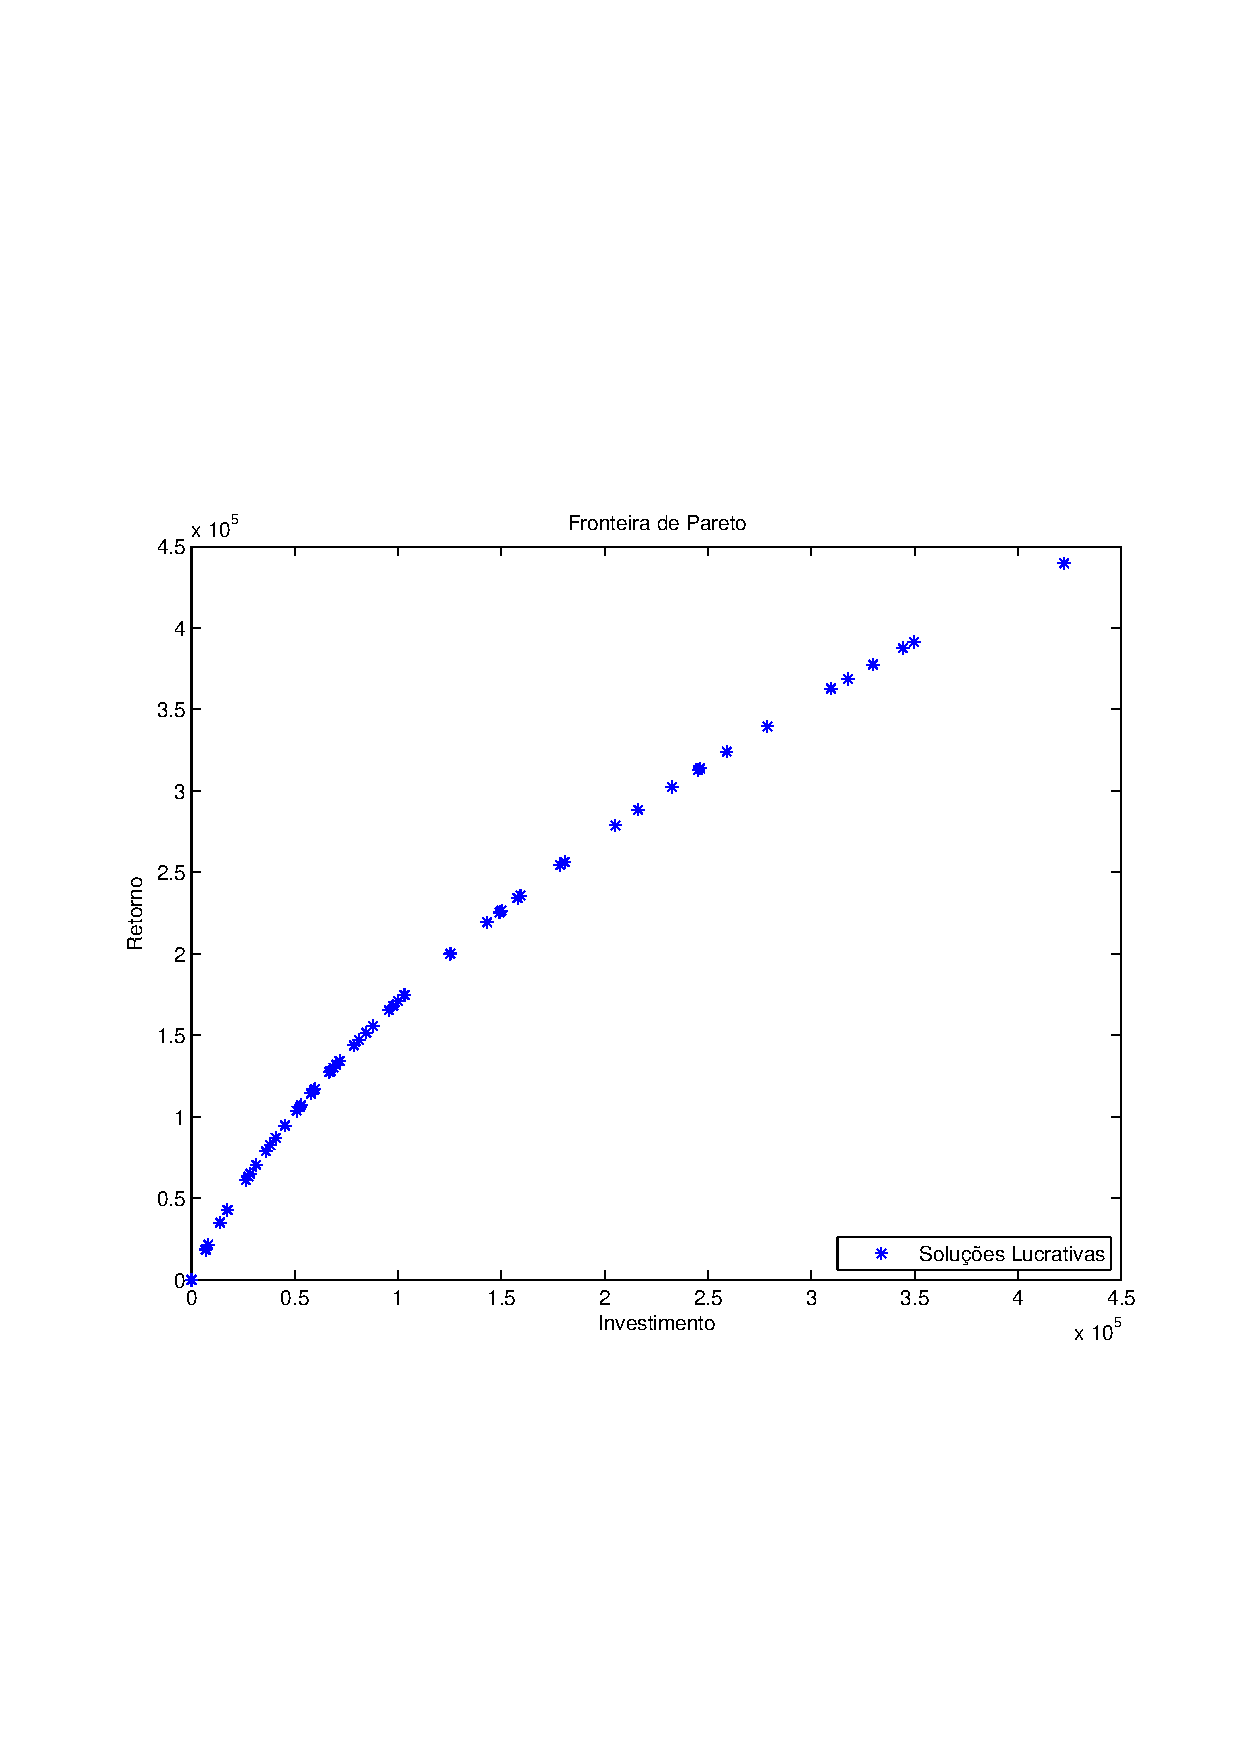
\includegraphics[width=12.0cm]{img/fronteira-lucro}
	\caption{Fronteira de Pareto para as soluções lucrativas do modelo apresentado na Equação \ref{eq:modelo}.}
	\label{fig:fronteira}
\end{figure}

Algumas observações podem ser feitas de acordo com as soluções encontradas. A solução com menor lucratividade é a primeira em negrito. Ela é a solução para o qual o investimento foi minimizado exclusivamente. Por ser muito baixa, ela certamente não deve ser interessante para o tomador de decisão do laticínio. As duas soluções com maior lucratividade, em negrito na tabela, possui um retorno por volta de $ 7,65 \cdot 10^4 $ unidades monetárias.

A média do lucro das soluções Pareto ótimas encontras possui uma média amostral de $ 5,336 \cdot 10^4 $ e desvio padrão amostral de $  2,1931e \cdot 10^4 $ unidades monetárias. A Figura \ref{fig:hist-lucro} apresenta a distribuição do lucro, em unidades monetárias, das soluções não dominadas lucrativas encontradas. Pode-se observar que a maioria das soluções se concentram no intervalo próximo do lucro máximo obtido. Por outro lado, existem um número considerável de soluções com lucros menores e que podem ser adotadas, caso o poder de investimento da empresa não seja muito alto.

\begin{figure}
	\centering
	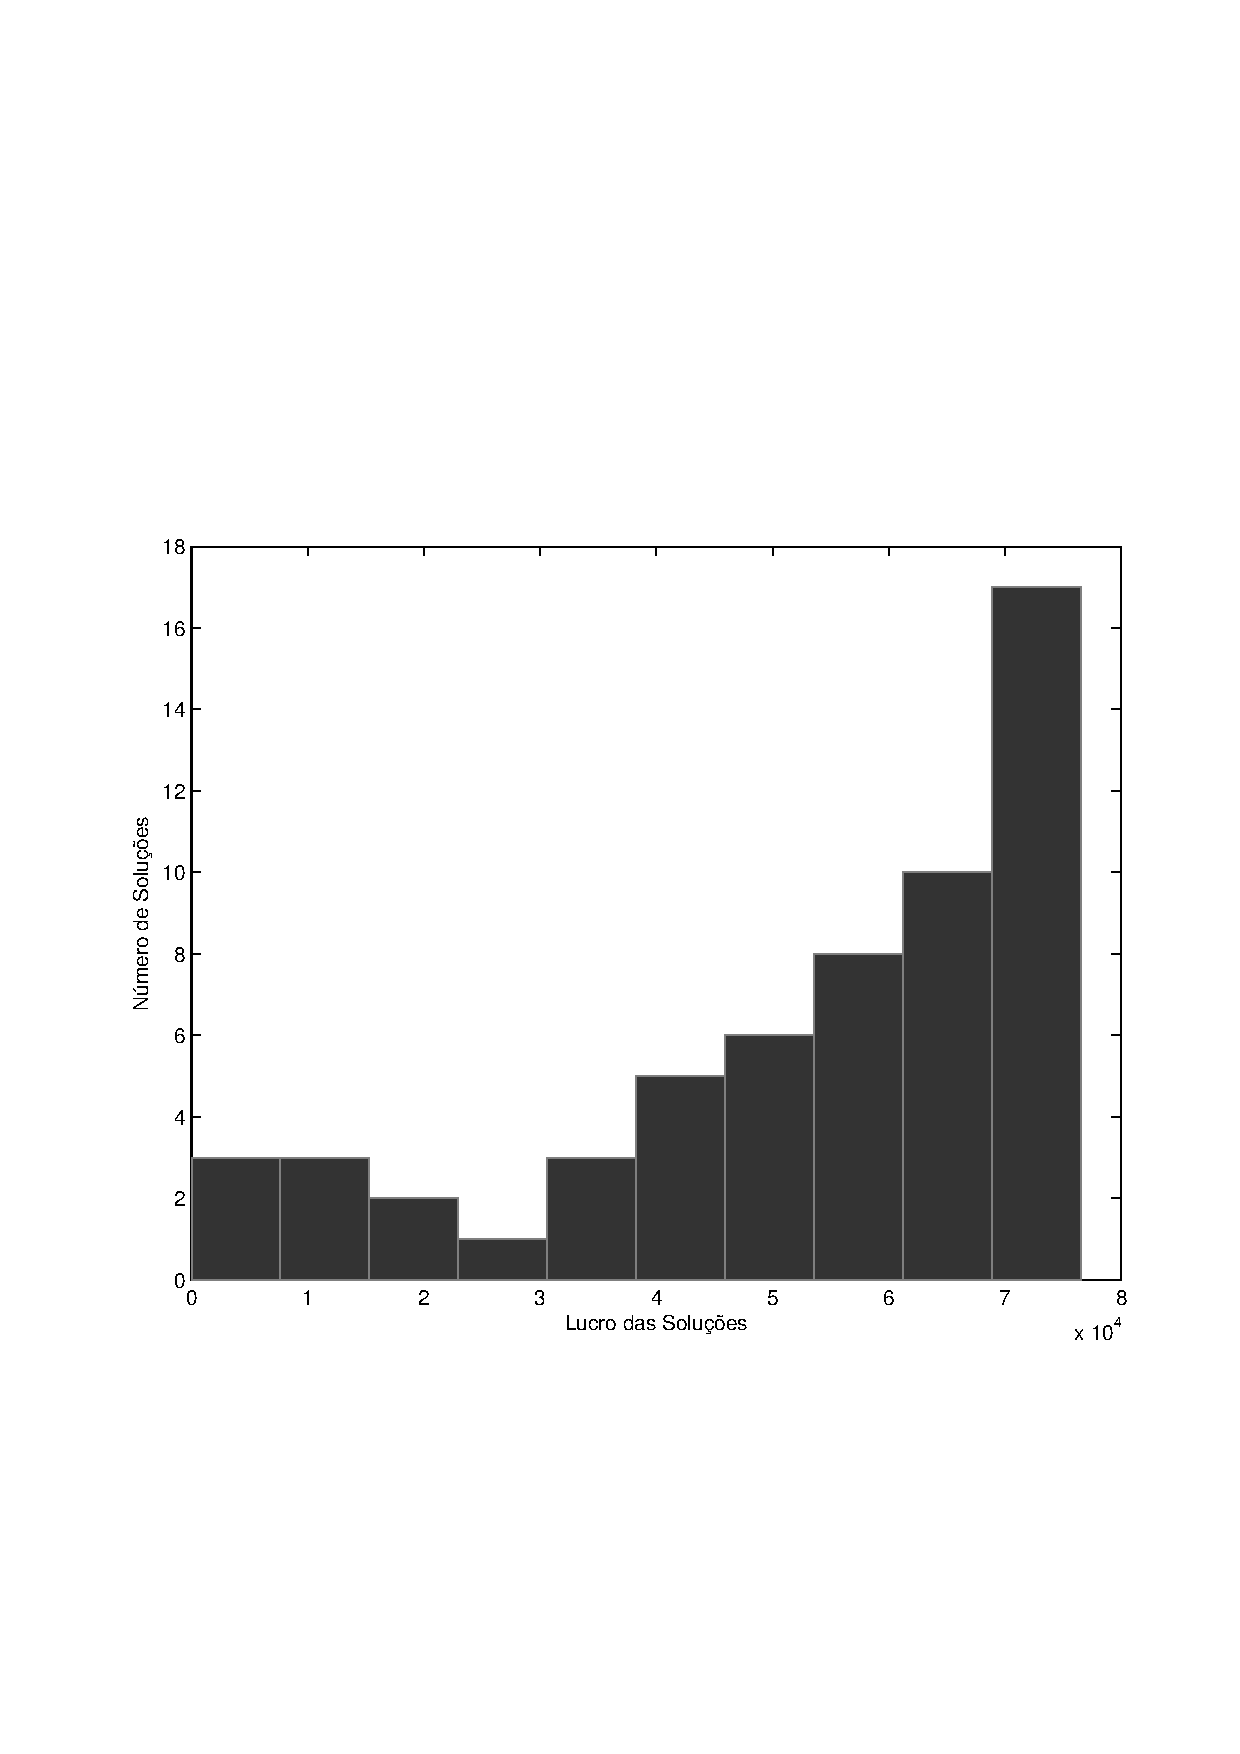
\includegraphics[width=12.0cm]{img/hist-lucro}
	\caption{Distribuição do lucro das soluções apresentadas na Figura \ref{fig:fronteira}.}
	\label{fig:hist-lucro}
\end{figure}

Outras considerações para o decisor podem ser feitas através da análise de sensibilidade das soluções. Porém, devido à questão de espaço, isto não é feito neste trabalho.

\section{Conclusões}
\label{sec:conclusao}

Este trabalho apresentou uma abordagem multiobjetivo que visa determinar a quantidade de produtos de um laticínio a ser produzida de modo maximizar o valor das vendas e minimizar o custo com investimentos. O modelo de variáveis reais, que possui uma função objetivo linear e a outra quadrática com restrições puramente lineares, foi solucionado via método $ P_{\lambda} $ em um processo de Monte Carlo, no qual as soluções não dominadas e diferenciadas por uma chave foram armazenadas em uma tabela hash.

Da amostra do conjunto Pareto ótimo encontrada, foram excluídas as soluções que geram prejuízo, ficando somente aquelas lucrativas. Uma análise destas soluções foram feitas através de gráficos e estatísticas. Deste modo, foi possível observar o comportamento das soluções de acordo com o valor investido e o retornado.

O conjunto com soluções ótimas, no sentido multiobjetivo, produto final deste trabalho, deve ser analisado pelo tomador de decisão para que escolha a solução que melhor se adeque à capacidade de investimento do laticínio, gerando assim o lucro maior possível.

\bibliography{referencias}
\bibliographystyle{abnt-alf}

\end{document}